\documentclass[tikz,border=8pt]{standalone}
\usepackage{amsmath}
\definecolor{bgcol}{HTML}{171D2B}
\definecolor{acc}{HTML}{F7B538}
\begin{document}
\pagecolor{bgcol}
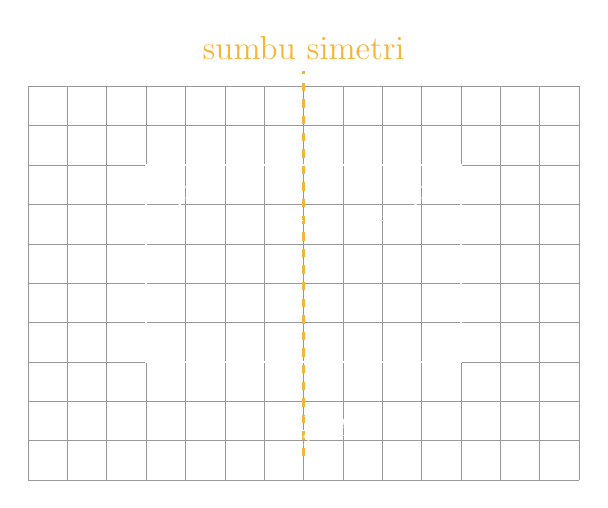
\begin{tikzpicture}[line width=1pt, text=white, font=\large]
  % Grid halus
  \draw[very thin, black!40] (-1.5,-1.5) grid[step=0.5] (5.5,3.5);
  % Segiempat ABCD
  \coordinate (A) at (0,0); \coordinate (B) at (0,2.5);
  \coordinate (C) at (4,2.5); \coordinate (D) at (4,0);
  \draw[white] (A) -- (B) -- (C) -- (D) -- cycle;
  \node[above left]  at (B) {$B$};
  \node[above right] at (C) {$C$};
  \node[below right] at (D) {$D$};
  \node[below left]  at (A) {$A$};
  % Sumbu simetri
  \draw[acc, dashed] (2,-1.2) -- (2,3.7);
  \node[acc, above] at (2,3.7) {sumbu simetri};
  % Titik P dan bayangan P'
  \coordinate (P) at (0.8,1.8);
  \fill[white] (P) circle (2pt); \node[above left] at (P) {$P$};
  \coordinate (Pp) at (3.2,1.8);
  \fill[white] (Pp) circle (2pt); \node[above right] at (Pp) {$P'$};
  \draw[white, thin, dotted] (P) -- (Pp);
  \node[below, text=white] at (2,-0.55) {\small $a=\tfrac{1}{2}AB$};
\end{tikzpicture}
\end{document}
